

\subsection{Introduction}

We have seen two main asymmetric primitive in the last lectures - RSA and Discrete Log Problem. In RSA problem, we work in ${Z_N}^*$ where $N=pq$ and p,q are prime number. The main assumption is that, given N and it's factor p and q, we can have a pair of public key e and secret key d such that $X^e mod N$ doesn't reveal any information about d. The Discrete Log Problem works in ${Z_p}^*$ for a prime P and the assumption is given $g^x mod p$, where g is a generator, we can't recover x. In both of the above primitives, we need to increase the group size considerably to provide better security guarantee. eg to provide 256-bit security, the group size needs to be 15360 bit size. The increase in group size leads to increase in  bandwidth, storage and computational time. This lead to the development of cryptographic primitives based on Elliptic Curve, which had group size just twice larger than the security parameter. Elliptic Curve are now the go-to state of the art practice and driven by the fact that RSA and Discrete Log Problem has become slower and slower over the years.

Elliptic Curves are discrete log-based system. They use a new kind of group defined relative to a finite field. Finite field allows basic operations like Addition, Multiplication, Subtraction and Division. Thus, finite fields have two operation and everything has inverse under both operations. An example of finite field group is integer modulo p which is denoted by $F_p$ or $GF(p)$. Elliptic Curves will use curves over $F_p$. 

\newtheorem{df}{Definition}
\begin{df}
Elliptic Curves are defined as by the set of x,y points in $F_p$ defined by the equation 
\bnm
E={(x,y) \mid y^2 = x^3+ax+b\mod p}
\enm 
where a,b are fixed values also from $F_p$, plus one special point called Point of Infinity $\cal O$
\end{df}

It is also required $E$ to be non-singular. In other words,
the partial derivatives shouldn't vanish simultaneously for any point
on $E$. This is equivalent to requiring that the
equation $x^{3}+Ax+B=0$ has no multiple roots. Thus, solving the above condition leads to the following lemma.

\begin{lemma}
 E is non singular if and only if $4A^{3} + 27B^{2}$ is not equal to zero
\end{lemma}

The \figref{fig:plot} shows the Eliptic Curve plot for the curve with A = -5 and B = 5. The graph is symmetric over the x-axis. It should be noted that graph consists of real points on other hand finite field consist of some points on this graph. For example few points on this graph are (1,1) and (1,-1) are points of $F_5$ of this graph.


\begin{figure}[!h]
\begin{adjustbox}
{center}
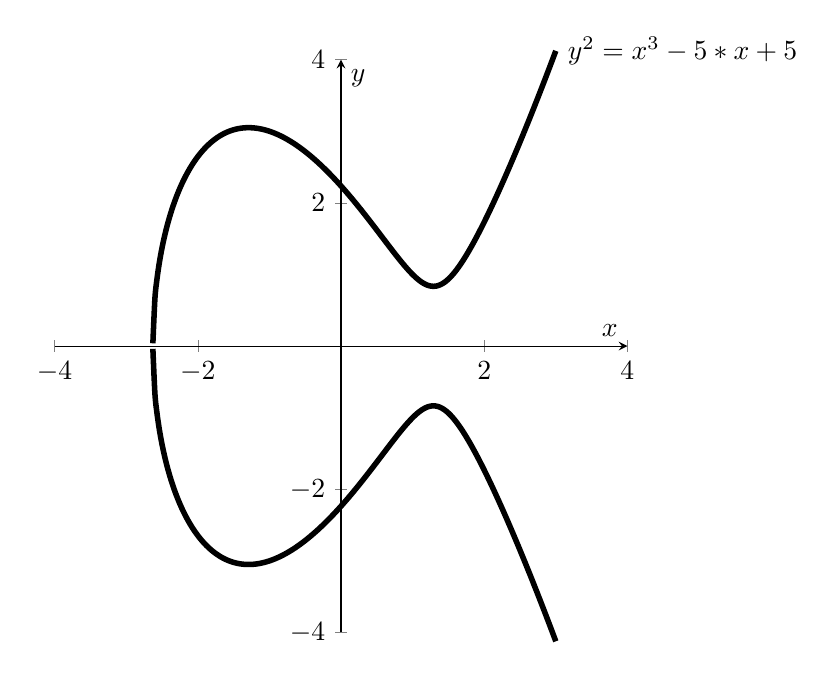
\begin{tikzpicture}
	
        \begin{axis}[
            xmin=-4,
            xmax=4,
            ymin=-4,
            ymax=4,
            xlabel={$x$},
            ylabel={$y$},
            scale only axis,
            axis lines=middle,
            % set the minimum value to the minimum x value
            % which in this case is $-\sqrt[3]{7}$
             domain=-2.7427:3,     % <-- works for pdfLaTeX and LuaLaTeX
%            domain=-1.91293118:3,   % <-- would also work for LuaLaTeX
            samples=200,
            smooth,
            % to avoid that the "plot node" is clipped (partially)
            clip=false,
            % use same unit vectors on the axis
            axis equal image=true,
        ]
            \addplot [line width=2pt,black] {sqrt(x^3-5*x+5)}
                node[right] {$y^2=x^3-5*x+5$};
            \addplot [line width=2pt,black] {-sqrt(x^3-5*x+5)};
        \end{axis}
    \end{tikzpicture}
    \end{adjustbox}
      \caption{Plot for $y^2=x^3-5*x+5$}
        \label{fig:plot}

\end{figure}

\subsection{Elliptic Curve Group Operation.} A Group is a set G along with a binary operation associated with this group. This operation should have certain set of properties. It should be closed and associative. Also, the group must contain an identity element and also have an inverse within the group for each element. The abelian groups also follow commutative property. 

\begin{figure}
\includegraphics{ecc/ec_group_operations.pdf}
\caption{Geometric Representation of Elliptic Curve Group Operation}
 \label{fig:oper}
\end{figure}

All the points on any elliptic curve form an abelian group. The rule associated with this group can be explained using \figref{fig:oper}. It is assumed that every vertical line passes through the neutral element or point of infinity $ \cal O$ as shown in the figure. Inverse element of a point P, $P^{-1}$ is the point of intersection of vertical line through P and the curve. The group operation for Elliptical Curve is called Point Addition and denoted by $P+Q$, where P and Q are points on the curve. Let $\diamond$ operator on points P and Q on the curve represent the intersection point of the line joining P and Q and the curve. Then the point addition can be represented as $\cal O \diamond (P \diamond Q)$. In other words, it represents the  intersection of the vertical line through $P \diamond Q$ and the curve. The doubling of P, i.e P+P, is represented by similarly by taking the intersection of tangent of P and the curve and drawing a vertical line through that point to get it's intersection with the curve as shown in figure \figref{fig:oper}.

\paragraph{Algebraic Representation.} We can represent the group operation algebraically as well for finite fields. The slope for the line between point P(x1,y1) and Q(x2,y2) is $D = \frac{y2-y1}{x2-x1} \mod p$. Thus the equation for the line will be  $y = D(x-x1) + y1 mod p$. To find the intersection of the line with the curve, we will substitute the value of y to get ${D(x-x1) + y1}^2 = x^3 + ax + b \mod p$. The solution of this equation are x1 , x2 and $x3 = D^2-x1-x2 \mod p$, which gives $y3 = D(x3-x1) + y1 \mod p$. Thus, the pseudo code to get the Point Addition between two points P and Q is given in \ref{algo}. The pseudo code also handles the corner cases where the P or Q is $\cal O$, then the result will the corresponding other point. In case the points are symmetric, the point addition will return $\cal O$. Finally in case of point doubling, the slope with the slope of tangent at that point.

\makeatletter
\def\BState{\State\hskip-\ALG@thistlm}
\makeatother

\begin{algorithm}
\caption{PointAddition Algorithm with input P(x1,y1) and Q(x2,y2) }\label{algo}
\begin{algorithmic}[1]
\Procedure{PointAddition}{}
\If {$P = \cal O$}
return Q
\EndIf
\If {$Q = \cal O$}
return P
\EndIf
\If {$x1 = x2$ and $y1 = -y2$}
return $\cal O$
\EndIf
\If{$x1 = x2$ and $y1 = y2$}
\State $D \gets \frac{3*{x1}^2+a}{2*y1} \mod p$
\Else 
\State $D \gets \frac{y2-y1}{x2-x1} \mod p$
\EndIf
\State $x3 \gets D^2-x1-x2 \mod p$
\State $y3 \gets D(x3-x1) + y1 \mod p$
\State return (x3,-y3)
\EndProcedure
\end{algorithmic}
\end{algorithm}

Interestingly, the point addition is a abelian group operation as it satisfies all four properties for group operation plus commutative property.
\begin{itemize}
\item Closure Property. P+Q lies on the curve for all P and Q, as discussed earlier.
\item Associative Property. (P+Q)+R = P+(Q+R)
\item Inverse Property. $P + P^{-1} = \cal O $ where $P^{-1} = (-x,y)$ for P=(x,y). Also ${\cal O}^{-1} = \cal O$. Since line passing through P and $P^{-1}$ is vertical line, it passes through $\cal O$.
\item Identity Property. P+$\cal O$ = P, as the vertical line intersects the inverse point $P^{-1}$, and vertical line through $P^{-1}$ intersect $P$. Thus point of infinity is identity for the group.
\item Commutative Property. P+Q = Q +P, as the line passing through P and Q will be same in both case.
\end{itemize}

\paragraph{Scalar Multiplication.} Scalar multiplication $nP$ is equivalent to adding P to itself n times. This is analogous to exponentiation in $Z_p$ and can be computed by point double and add algorithm similar to square and multiply in case of integers. We can also pick generator P that defines cyclic subgroup of E such that $0P, 1P, 2P, 3P \dots qP$ all lies on the curve. It should be the case the subgroups are large.

\paragraph{Building Elliptic Curve Groups.} Earlier people use to find suitable curves by a deterministic algorithm that picks a large prime p and pick values a and b to define a curve. Then check using Schoof algorithm the size of group if it is prime for security reasons. Finally pick a point P to be generator. This process was very slow. Recently, these curves and generator P have been standardized instead. Some examples are NIST curves, Curve25519 etc. 







